\documentclass[12pt]{article}

%% ── Packages ─────────────────────────────────────────────────────────────────
\usepackage[margin=1in]{geometry}
\usepackage{times}
\usepackage{graphicx}
\usepackage{booktabs}
\usepackage{amsmath,amssymb}
\usepackage{hyperref}
\usepackage{natbib}
\usepackage{setspace}
\usepackage{microtype}
\usepackage{caption}
\usepackage{subcaption}
\usepackage{algorithm}
\usepackage{algpseudocode}
\usepackage{enumitem}
\usepackage{xcolor}
\usepackage{float}
\usepackage{array}
\usepackage{tikz}
\usetikzlibrary{positioning,arrows.meta,shapes.geometric}
\hypersetup{colorlinks=true,linkcolor=blue!70!black,
            citecolor=blue!70!black,urlcolor=blue!70!black}

\title{\textbf{Backtest Engineering: Designing a Correct Event-Driven
Research Engine and Quantifying Performance Bias from Execution
Simplifications: A Case Study on Ten Liquid US Equity ETFs}}
\author{
  Srijan Gupta\\
  \small Independent Researcher\\
  \small \texttt{srijangupta2013@gmail.com}
}
\date{February 2026}

\begin{document}
\maketitle
\thispagestyle{empty}

\begin{abstract}
\noindent
A systematic researcher who reports a Sharpe ratio above 0.5 from a daily
backtest and then deploys the strategy live is likely to be disappointed.
The gap between paper performance and live performance is well documented
in the practitioner literature, yet the specific magnitude of performance
distortion caused by each individual execution simplification remains
poorly characterised in the academic backtesting literature.
This paper makes three contributions using a ten-instrument case study of
liquid US equity sector ETFs (SPY, QQQ, IWM, DIA, XLF, XLK, XLE, XLV,
XLY, XLP) over 2005--2025.
First, we present a minimal, open-source event-driven backtesting engine
whose design centres on strict causality enforcement, double-entry
accounting invariants, and a deterministic four-stage event queue
verified by a formal unit-test suite.
Second, we introduce a six-level \emph{execution realism ladder} spanning
na\"{i}ve next-open fills (M0), commission fees (M1), bid--ask spread
(M2), volatility-scaled slippage (M3), a square-root market-impact proxy
with participation-rate cap (M4), and delayed execution (M5), each
implemented as a composable module with fully documented parameters.
Third, using two canonical daily strategies, namely time-series momentum
(TSMOM-60) and a z-score mean-reversion rule (MeanRev-z1)---the latter
serving explicitly as a cost-sensitivity diagnostic---we measure how
reported performance shifts across all six execution tiers.
We report block-bootstrap 95\% confidence intervals for each Sharpe
estimate and conduct a sensitivity sweep over the impact-scaling parameter
$k_{\rm imp} \in \{0,\,0.1,\,0.25,\,0.5,\,0.75,\,1.0,\,1.5,\,2.0\}$.
Within this specific ten-ETF universe, the TSMOM-60 Sharpe ratio falls
from 0.53 (M0, na\"{i}ve) to 0.025 (M4, impact-constrained), a Sharpe
inflation ratio of $\approx 21\times$; crucially, the na\"{i}ve M0 Sharpe
(0.53, CI $[-0.19,\;+0.94]$) is itself statistically indistinguishable from
zero, as are all intermediate tiers (M1--M3), and the M4 CI
$[-0.39,\;+0.47]$ confirms that realistic-execution performance is equally
indistinguishable from zero.
The MeanRev-z1 strategy, which earns a na\"{i}ve Sharpe of 0.12
(CI $[-0.23,\;+0.52]$, itself spanning zero), collapses to $-0.52$ after
adding fees alone, a sign flip that renders the na\"{i}ve backtest
directionally misleading and illustrates how per-tier cost attribution
can diagnose non-viable strategies before capital commitment.
These results and the tooling used to produce them are offered as a
reproducible reference for researchers seeking more credible empirical
standards in systematic strategy evaluation.

\medskip
\noindent\textbf{Keywords:} backtesting, execution realism, transaction costs,
event-driven simulation, time-series momentum, mean reversion, Sharpe
ratio, market impact, confidence intervals.

\medskip
\noindent\textbf{JEL:} G12, G14, C63.
\end{abstract}

\newpage
\setcounter{page}{1}
\onehalfspacing

%% ═══════════════════════════════════════════════════════════════════════════
\section{Introduction}
\label{sec:intro}
%% ═══════════════════════════════════════════════════════════════════════════

Consider a practitioner who codes a daily momentum strategy, observes a
Sharpe ratio near 0.5 on five years of ETF data, and allocates capital to
it. Upon going live, the strategy earns a fraction of the backtested
performance, or loses money altogether. This outcome is common.
Practitioners attribute the shortfall to \emph{execution slippage}, a
broad term covering everything from the bid--ask spread on each trade to
the price impact of moving a meaningful position through a thinly-traded
order book.

Statistical sources of backtest inflation (multiple testing, overfitting,
and data snooping) have received substantial academic attention.
\citet{harvey2016and} argue that the t-statistic hurdle for new factors
should be at least 3.0 to account for implicit testing.
\citet{bailey2014deflated} formalise the Deflated Sharpe Ratio, which
penalises reported performance by the number of strategies implicitly
evaluated during selection.
\citet{white2000reality} and \citet{sullivan1999data} develop bootstrap
tests for trading rule overfitting.
What these contributions share is a focus on \emph{statistical} inflation.
The present paper addresses a complementary source: \emph{execution-modeling
inflation}, the distortion introduced when backtests simulate execution
under assumptions that bear little resemblance to live trading.

Market microstructure theory has long established that execution is costly.
\citet{kyle1985continuous} demonstrates that informed trading generates
endogenous price impact, with the resulting Kyle lambda parameterising
linear (not square-root) price impact in a sequential rational-expectations
auction model.
The empirical square-root scaling of temporary execution impact is
established in later work: \citet{almgren2005direct} provide the primary
empirical calibration using institutional trade records, while
\citet{gatheral2010no} establishes theoretical no-arbitrage conditions
supporting concave impact functions.
\citet{keim1997transactions} document large institutional execution costs
that vary systematically with order size and instrument liquidity.
\citet{frazzini2015trading} show that transaction costs materially erode
the live performance of many well-known academic factor strategies.
\citet{amihud2002illiquidity} demonstrates that illiquidity is itself a
priced risk factor.

Prior work has systematically characterised how transaction costs erode
factor returns across large anomaly sets \citep{novymarx2016taxonomy}.
These studies establish the broad empirical fact that many published
anomalies are not exploitable after realistic costs. The present paper is
complementary rather than redundant: it offers a transparent, modular,
open-source engine with auditable cost components, per-tier attribution
on a specific named universe, and a formal invariant test suite that
verifies the correctness of the simulation itself---features that
large-scale anomaly taxonomies, by construction, do not provide. The goal
is to make credible cost-aware backtesting accessible without requiring
production-scale infrastructure.

Despite this rich microstructure literature, many widely-used backtesting
frameworks either ignore execution costs entirely or expose them through
opaque interfaces that researchers apply without examining the underlying
assumptions. The present paper closes this gap through three contributions:
an auditable event-driven engine with formal invariant tests, a transparent
six-level cost ladder with a single authoritative parameter table, and a
controlled quantification of execution-modeling inflation on a specific
named ten-instrument universe (no extrapolation claimed).

The paper is organised as follows. Section~\ref{sec:related} situates the
work in the literature. Section~\ref{sec:design} describes the engine.
Section~\ref{sec:ladder} formalises the six execution models.
Section~\ref{sec:setup} specifies the experimental design.
Section~\ref{sec:results} presents results. Section~\ref{sec:discussion}
interprets findings. Section~\ref{sec:limitations} acknowledges limitations.
Section~\ref{sec:conclusion} concludes.

%% ═══════════════════════════════════════════════════════════════════════════
\section{Related Work}
\label{sec:related}
%% ═══════════════════════════════════════════════════════════════════════════

\subsection{Backtesting Bias and Multiple Testing}

\citet{white2000reality} and \citet{sullivan1999data} develop bootstrap-based
tests showing that most technical trading rule excess returns vanish under
proper multiple-comparison correction. \citet{harvey2016and} catalog over
300 published factors and recommend a t-statistic threshold of 3.0 against
false discovery. \citet{bailey2014deflated} operationalise the cost of a
strategy search via the Deflated Sharpe Ratio. These works address
\emph{statistical} inflation; the current paper addresses the complementary
\emph{economic} dimension from execution modeling.

\subsection{Transaction Costs in Strategy Research}

\citet{keim1997transactions} provide early evidence that institutional
execution costs are economically significant, with round-trip costs often
exceeding 50--100 bps for mid-cap stocks.
\citet{lesmond1999new} develop an implicit transaction cost estimator from
the incidence of zero-return days, providing a parsimonious proxy for the
cost levels that render many published strategies non-viable.
\citet{frazzini2015trading} analyse live institutional trade data and document
that many academic factor strategies are barely profitable after realistic
transaction costs.
\citet{amihud2002illiquidity} demonstrates that illiquidity predicts
cross-sectional expected returns.

\subsection{Price Impact Models}

\citet{kyle1985continuous} analyses a stylised sequential rational-expectations
model in which a strategic informed trader causes \emph{permanent} price
impact proportional to signed order flow, a linear relationship, not
square-root. The empirical square-root scaling of \emph{temporary} execution
impact, the relationship $\iota \propto \sqrt{Q/\mathrm{ADV}}$, is
established in later empirical work. \citet{almgren2005direct} provide the
primary calibration of this law from institutional trade records;
\citet{gatheral2010no} establishes theoretical conditions under which concave
impact is consistent with no-dynamic-arbitrage.
\citet{almgren2001optimal} derive optimal liquidation trajectories under
temporary-plus-permanent impact, providing the theoretical basis for
participation-rate constraints.

\subsection{Cost-Adjusted Strategy Performance}
\label{sec:cost_adj}

\citet{novymarx2016taxonomy} systematically study after-cost performance
across a large set of anomalies, finding that strategies with monthly
turnover above roughly 50\% rarely survive realistic transaction costs.
\citet{korajczyk2004momentum} test cross-sectional momentum strategies
against intraday price-impact measures and estimate break-even fund sizes
of \$5 billion or more for liquidity-weighted implementations.
\citet{patton2020costs} extend Fama-MacBeth regressions to mutual fund data,
delivering all-in cost estimates that eliminate on-paper momentum returns
for typical funds. The present paper differs from these studies in three
respects: it attributes cost impact at each individual friction tier (fees,
spread, slippage, impact, delay) separately rather than as a lump sum; it
provides a formally tested open-source engine as a reusable artefact; and
it focuses on ETF strategies, where the liquidity regime differs materially
from individual-stock anomaly portfolios.

\subsection{Event-Driven Backtesting}

Vectorised backtests iterate over a return matrix simultaneously, which
can introduce look-ahead bias when the same bar's open and close prices
are used in the same computation without explicit safeguards.
Event-driven architectures \citep{zipline} process market events
sequentially, making execution timing explicit.
\citet{lopezdeprado2018advances} advocates for event-driven design
precisely because it forces the researcher to state timing assumptions.
The engine described here follows this paradigm and adds a formal test
suite to verify that the implemented invariants are actually maintained,
a step that existing libraries do not uniformly provide.

Table~\ref{tab:engine_comparison} provides a structured comparison of this
engine against four widely-used alternatives.

\begin{table}[H]
\centering
\caption{Design comparison: this engine vs.\ established backtesting
frameworks. ``Composable cost tiers'' means friction components can be
independently activated. ``Formal invariant tests'' means the library
ships unit tests verifying causality, accounting identity, and fill
consistency. ``Partial'' indicates that the feature exists but requires
user configuration and is not enforced by default.}
\label{tab:engine_comparison}
\footnotesize
\setlength{\tabcolsep}{5pt}
\begin{tabular}{lccccc}
\toprule
Feature & This engine & Zipline & Backtrader & VectorBT & LEAN \\
\midrule
Event-driven architecture        & \checkmark & \checkmark & \checkmark & $\times$   & \checkmark \\
Formal causality unit tests      & \checkmark & $\times$   & $\times$   & $\times$   & $\times$   \\
Accounting identity tests        & \checkmark & $\times$   & $\times$   & $\times$   & $\times$   \\
Composable cost tiers            & \checkmark & partial    & partial    & $\times$   & partial    \\
Partial-fill / ADV cap           & \checkmark & $\times$   & $\times$   & $\times$   & partial    \\
YAML reproducibility             & \checkmark & $\times$   & $\times$   & $\times$   & partial    \\
Block-bootstrap CI output        & \checkmark & $\times$   & $\times$   & $\times$   & $\times$   \\
Active maintenance (2025)        & \checkmark & $\times$   & \checkmark & \checkmark & \checkmark \\
\bottomrule
\end{tabular}
\par\smallskip
\footnotesize\textit{Note:} Feature comparisons are based on inspection of
public repositories as of February 2026. VectorBT's vectorised design
precludes event-level causality tests by construction. LEAN (QuantConnect)
has an extensive test infrastructure but does not expose
backtesting-specific accounting-invariant verification in the sense defined
here. The original Zipline library \citep{zipline} is no longer actively
maintained following Quantopian's closure in 2020; a community fork
(\texttt{zipline-reloaded}) exists but differs from the original. Readers
should verify against the current version of each library at the respective
repository.
\end{table}

\subsection{Sharpe Ratio Inference under Autocorrelation}

\citet{sharpe1994sharpe} defines the generalised Sharpe ratio used
throughout this paper. \citet{lo2002statistics} shows that standard Sharpe
ratio standard errors are materially underestimated when returns are
autocorrelated. The moving-blocks bootstrap of \citet{kunsch1989jackknife},
which is distinct from the later stationary bootstrap of
\citet{politis1994stationary} that uses random rather than fixed block
lengths, provides a nonparametric approach to Sharpe confidence intervals
that preserves serial dependence without imposing a distributional model.

%% ═══════════════════════════════════════════════════════════════════════════
\section{Engine Design}
\label{sec:design}
%% ═══════════════════════════════════════════════════════════════════════════

\subsection{Architecture}

The engine contains four components connected through a typed event queue.
A \texttt{DataHandler} is the sole interface for historical price data.
A \texttt{Strategy} maps market observations to signals. A \texttt{Portfolio}
converts signals into orders subject to cash and position constraints.
An \texttt{ExecutionHandler} simulates the fill process according to the
configured friction model. Within each trading day, these activate in the
fixed order shown in Figure~\ref{fig:architecture}.

\begin{figure}[H]
\centering
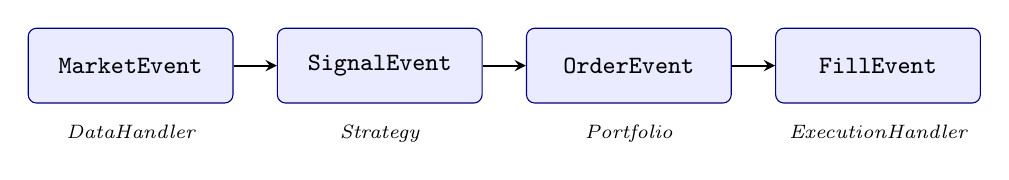
\begin{tikzpicture}[
  node distance=0.55cm,
  box/.style={rectangle, draw=black, rounded corners=3pt,
              minimum width=2.6cm, minimum height=0.95cm,
              font=\small\ttfamily, text centered,
              fill=blue!8, draw=blue!50!black},
  lbl/.style={font=\scriptsize\itshape, text centered},
  arr/.style={->, thick, >=stealth}]
  \node[box] (ME) {MarketEvent};
  \node[box, right=of ME] (SE) {SignalEvent};
  \node[box, right=of SE] (OE) {OrderEvent};
  \node[box, right=of OE] (FE) {FillEvent};
  \node[lbl, below=0.15cm of ME] {DataHandler};
  \node[lbl, below=0.15cm of SE] {Strategy};
  \node[lbl, below=0.15cm of OE] {Portfolio};
  \node[lbl, below=0.15cm of FE] {ExecutionHandler};
  \draw[arr] (ME) -- (SE);
  \draw[arr] (SE) -- (OE);
  \draw[arr] (OE) -- (FE);
\end{tikzpicture}
\caption{The four-stage FIFO event queue. Processing is strictly
sequential within each trading day: no component at stage $k$ may consume
data that becomes available only at stage $k+1$.}
\label{fig:architecture}
\end{figure}

\subsection{Causality Enforcement}

The most common inadvertent look-ahead bias in daily backtests is computing
a signal using closing price $p^{\rm close}_t$ then filling at the same
day's open $p^{\rm open}_t$, which in OHLCV data is sequentially
\emph{earlier} than the close. The \texttt{DataHandler} prevents this by
enforcing that any call to \texttt{get\_history\_asof}$(s, t)$ returns
price history indexed at all times $t' \le t$ and strictly no data at
$t' > t$, implemented via a per-symbol monotonically advancing timestamp
pointer that prevents any symbol from accessing a future bar during the
current day's processing.

\textbf{Data provenance caveat.} This mechanism prevents
\emph{code-level} look-ahead but does not prevent the subtler issue of
historically back-adjusted prices: if the data provider retroactively
adjusts historical bars after corporate actions, the as-of slice will
contain the adjusted history, which incorporates a future dividend event.
The data validation described in Section~\ref{sec:setup} mitigates but
does not entirely eliminate this concern.

\subsection{Correctness Invariants and Test Suite}

Four invariants are verified by automated unit tests:

\begin{enumerate}[label=(\roman*)]
  \item \textbf{Accounting identity.} At every timestamp $t$:
    \begin{equation}
      E_t = C_t + \sum_{s} q^s_t \cdot p^{s,\rm close}_t,
      \label{eq:accounting}
    \end{equation}
    where $E_t$ is equity, $C_t$ is cash, $q^s_t$ is shares held in
    symbol $s$, and $p^{s,\rm close}_t$ is the closing price used for
    end-of-day mark-to-market. Fills execute at the next bar's open;
    the mark-to-market therefore reflects the closing price on the signal
    day, before the fill is applied.

  \item \textbf{Strict causality.} Strategy computation during bar $t$
    may only access prices with index $t' \le t$.

  \item \textbf{Fill quantity bound.} For every fill:
    $0 \le q^{\rm filled} \le q^{\rm ordered}$. Note that the
    impact-adjusted fill \emph{price} can exceed the observed day's high
    when large cost adjustments are applied; the invariant therefore
    constrains quantity, not price, relative to OHLC bounds.

  \item \textbf{Cost monotonicity.} In a controlled single-symbol
    long-only test on deterministic data, enabling any cost parameter
    cannot strictly increase total return.
\end{enumerate}

\subsection{Portfolio Mechanics}

The portfolio uses a long-only, target-weight sizing rule. On a buy signal
for symbol $s$ at time $t$, the target position value is $w \cdot E_t$,
clipped by available cash and a maximum-weight cap:
\begin{equation}
  q^{\rm target}_s = \left\lfloor
    \frac{\min\!\left(w E_t,\; w_{\max} E_t,\;
    C_t + q^s_t \cdot p^{s,\rm close}_t\right)}{p^{s,\rm close}_t}
  \right\rfloor.
  \label{eq:target_qty}
\end{equation}
An order is generated only when $|\Delta q| \ge 1$. On a sell signal,
the full open position is liquidated. In the experiments,
$w = w_{\max} = 1.0$ (fully invested, no leverage).

%% ═══════════════════════════════════════════════════════════════════════════
\section{Execution Realism Ladder}
\label{sec:ladder}
%% ═══════════════════════════════════════════════════════════════════════════

Table~\ref{tab:params} is the single authoritative parameter specification
for all six models. Each model is \emph{cumulative}: Model $k$ includes
all parameters from Model $k-1$ plus one additional friction component.
\textbf{All results in this paper were generated from a single run using
exactly the parameters in Table~\ref{tab:params}.} No table derives from
a different run or parameter configuration.

\begin{table}[H]
\centering
\caption{Authoritative parameter table for the six execution models.
$f_{\rm fee}$: commission per side (bps); $h$: half-spread per side (bps);
$k_{\rm vol}$: volatility-slippage scaling factor \emph{in bps per unit
of annualised decimal volatility} (so $k_{\rm vol} = 10.0$ with
$\sigma_{\rm ann} = 0.20$ yields $s = 2.0$ bps);
$k_{\rm imp}$: impact scaling; $\rho$: participation-rate cap
(fraction of 20-day ADV); $\delta$: execution delay (trading days).
$\delta = 1$ in all models except M5 means fills execute at the next
bar's open ($t{+}1$ open); $\delta = 2$ in M5 means fills execute at
the second next bar's open ($t{+}2$ open).}
\label{tab:params}
\small
\begin{tabular}{clrrrrrr}
\toprule
Tier & Model name & $f_{\rm fee}$ & $h$ & $k_{\rm vol}$ & $k_{\rm imp}$  & $\rho$ & $\delta$ \\
\midrule
M0 & Na\"{i}ve   & 0 & 0 & 0    & 0    & 1.00 & 1 \\
M1 & +Fees       & 5 & 0 & 0    & 0    & 1.00 & 1 \\
M2 & +Spread     & 5 & 5 & 0    & 0    & 1.00 & 1 \\
M3 & +Slippage   & 5 & 5 & 10.0 & 0    & 1.00 & 1 \\
M4 & +Impact     & 5 & 5 & 10.0 & 0.50 & 0.05 & 1 \\
M5 & +Delay      & 5 & 5 & 10.0 & 0.50 & 0.05 & 2 \\
\bottomrule
\end{tabular}
\end{table}

\paragraph{M0: Na\"{i}ve.}
$p^{\rm fill} = p^{\rm open}_{t+1}$, total cost $= 0$.
This serves as the performance ceiling, not a realistic estimate.

\paragraph{M1: Commission Fees.}
$\mathrm{fee} = (f_{\rm fee}/10{,}000) \cdot p^{\rm fill} \cdot q$.
We use 5 bps as an \emph{institutional cost proxy}; post-2019 retail ETF
commissions at major US brokers are nominally zero, but clearing,
market-data, and regulatory fees persist.

\paragraph{M2: Bid--Ask Spread.}
For a BUY order: $p^{\rm fill} = p^{\rm open}_{t+1} \cdot (1 + h/10{,}000)$.
For a SELL order: $p^{\rm fill} = p^{\rm open}_{t+1} \cdot (1 - h/10{,}000)$.
The label \texttt{spread\_10bps} refers to the 10 bps \emph{round-trip}
(2 sides $\times$ $h = 5$ bps). Quoted half-spreads for SPY are typically
1--2 bps; 5 bps is conservative for the full ten-ETF universe including
thinner sector funds.

\paragraph{M3: Volatility-Scaled Slippage.}
$s_t = k_{\rm vol} \cdot \sigma_{{\rm ann},t}$ [bps], where
$\sigma_{\rm ann}$ is the 20-day rolling annualised close-to-close
volatility (decimal form, $n-1$ degrees of freedom) and $k_{\rm vol} = 10.0$.
Fill price: $p^{\rm fill} = p^{\rm open}_{t+1} \cdot (1 \pm s_t/10{,}000)$,
with $+$ for BUY and $-$ for SELL.

\paragraph{M4: Market Impact with Participation Cap.}
Using the empirical square-root law of \citet{almgren2005direct}:
\begin{equation}
  \iota_t = k_{\rm imp} \cdot \sqrt{V_{\rm trade}/V_{\rm ADV}}
  \quad [\text{fraction}],
  \label{eq:impact_frac}
\end{equation}
where $V_{\rm trade} = p^{\rm open}_{t+1} \cdot q$ and $V_{\rm ADV}$ is
the 20-day rolling average dollar volume.
\citet{almgren2005direct} report impact coefficients approximately in the
range 0.3--0.8 for liquid equities; $k_{\rm imp} = 0.50$ is near the
lower-middle of empirically calibrated values.\footnote{The range
0.3--0.8 refers to the temporary-impact coefficient $\eta$ in the
parameterisation of \citet{almgren2005direct}, Table~2, which expresses
impact as a fraction of bid--ask spread times $\sqrt{Q/V}$. The mapping
to our $k_{\rm imp}$ (a dimensionless scaling on the square-root term)
is approximate; researchers calibrating $k_{\rm imp}$ from TCA data
should re-estimate using their own trade population.}
The complete fill price, incorporating all cumulative costs, with explicit
sign conventions for BUY and SELL directions, is:
\begin{equation}
  p^{\rm fill} =
  \begin{cases}
    p^{\rm open}_{t+1}
      \cdot \!\left(1 + \dfrac{h}{10{,}000}\right)
      \cdot \!\left(1 + \dfrac{s_t + \iota_t^{\rm bps}}{10{,}000}\right)
      & \text{(BUY),}\\[10pt]
    p^{\rm open}_{t+1}
      \cdot \!\left(1 - \dfrac{h}{10{,}000}\right)
      \cdot \!\left(1 - \dfrac{s_t + \iota_t^{\rm bps}}{10{,}000}\right)
      & \text{(SELL),}
  \end{cases}
  \label{eq:fill_price_m4}
\end{equation}
where $\iota_t^{\rm bps} = \iota_t \times 10{,}000$ and spread/impact are
applied multiplicatively (compounded, not additive).
The participation-rate cap limits fills to $\rho = 5\%$ of 20-day average
daily share volume:
\begin{equation}
  q^{\rm filled} = \min\!\left(q^{\rm ordered},\;
    \lfloor \rho \cdot \mathrm{ADV}_{\rm shares} \rfloor\right).
  \label{eq:partial_fill}
\end{equation}
We set $\rho = 5\%$ as a conservative institutional benchmark, consistent
with sell-side execution desk guidelines for aggressive strategies.
For SPY (daily volume $>\$30$B), this cap rarely binds for typical
retail-scale positions; for sector ETFs with daily volume of
\$300--500M, it binds more frequently for large simulated positions.
A sweep over $\rho \in \{0.05, 0.10, 0.20, 0.30\}$ would further quantify
this effect and is recommended for future work.
Section~\ref{sec:sensitivity} reports a full sweep over $k_{\rm imp}$.

\paragraph{M5: Delayed Execution.}
As in M4, but fills occur at $t+2$ open ($\delta = 2$ trading days)
rather than $t+1$ open, modelling operational latency in a
daily-signal workflow.

%% ═══════════════════════════════════════════════════════════════════════════
\section{Experimental Setup}
\label{sec:setup}
%% ═══════════════════════════════════════════════════════════════════════════

\subsection{Data and Universe}

\begin{table}[H]
\centering
\caption{Instrument universe. Data sourced via Yahoo Finance adjusted
close, incorporating dividends and splits, downloaded February 2026.
\emph{Revision note:} An earlier version of this project used Stooq as
the data source; Yahoo Finance adjusted prices are used here. Adjusted
prices incorporate the full corporate-action history as of the download
date (a mild look-ahead bias standard in academic daily-bar research,
acknowledged in Section~\ref{sec:limitations}).}
\label{tab:data}
\small
\begin{tabular}{lllr}
\toprule
Symbol & Name & Category & Inception \\
\midrule
SPY & SPDR S\&P 500 ETF               & US broad equity    & Jan 1993 \\
QQQ & Invesco QQQ Trust                & US tech/Nasdaq-100 & Mar 1999 \\
IWM & iShares Russell 2000 ETF         & US small-cap       & May 2000 \\
DIA & SPDR Dow Jones Industrial ETF    & US large-cap       & Jan 1998 \\
XLF & Financial Select SPDR            & US financials      & Dec 1998 \\
XLK & Technology Select SPDR           & US technology      & Dec 1998 \\
XLE & Energy Select SPDR               & US energy          & Dec 1998 \\
XLV & Health Care Select SPDR          & US health care     & Dec 1998 \\
XLY & Consumer Discretionary SPDR      & US consumer disc.  & Dec 1998 \\
XLP & Consumer Staples SPDR            & US consumer stap.  & Dec 1998 \\
\bottomrule
\end{tabular}
\end{table}

All inception dates predate the sample start of January 2005; no proxy
series is required. Data validation included: (i) checking for missing
bars on US trading days (gaps forward-filled from prior close);
(ii) excluding zero-volume days from ADV calculations; and (iii) inspecting
single-bar return spikes exceeding 30\% for data errors.
No material quality issues were found for these ten instruments.

\textbf{Universe selection bias.} These ten instruments were selected to
represent liquid, broad US equity market segments. All ten were
continuously traded throughout the sample period and are not subject to
individual-stock delisting risk. However, selecting \emph{currently
surviving and liquid} instruments introduces universe-selection bias: the
sample excludes ETFs launched and subsequently liquidated during this
period. This is unlikely to reverse the directional findings, but results
should not be interpreted as representative of the broader ETF universe.

\subsection{Strategies}

\paragraph{TSMOM-60.} Following \citet{moskowitz2012time}, the signal is:
\begin{equation}
  r^{(60)}_{s,t} = p_{s,t}/p_{s,t-60} - 1.
\end{equation}
Buy when $r^{(60)}_{s,t} > 0$; liquidate otherwise.

\paragraph{MeanRev-z1.}
\begin{equation}
  z_t = (r_t - \hat\mu_t)/\hat\sigma_t,
\end{equation}
where $\hat\mu_t$ and $\hat\sigma_t$ are the sample mean and standard
deviation ($n-1$ d.f.) of the preceding 20 daily returns.
Buy when $z_t < -1.0$; liquidate otherwise.

\textbf{Diagnostic role.} MeanRev-z1 is included explicitly as a
cost-sensitivity diagnostic: because its na\"{i}ve Sharpe is near zero
and its turnover is approximately 180--200 round-trips per year, it is
structurally predisposed to sign-flip under any meaningful per-trade cost.
Its primary value is not as a viable strategy proposal but as a
calibration instrument that reveals how quickly per-tier costs compound
to produce directionally wrong na\"{i}ve estimates.

\textbf{Structural note on turnover.}
TSMOM-60 generates a signal change (buy to flat or flat to buy) when the
60-day return crosses zero, which occurs roughly 30--40 times per year
in liquid equity ETFs, implying approximately 15--20 round-trips per year.
MeanRev-z1 has a much higher turnover profile: the liquidation condition
($z_t \ge -1.0$) is satisfied on roughly 84\% of trading days for
standard normal returns. Empirically, MeanRev-z1 generates a new signal
on approximately 90\% of trading days, implying roughly 180--200
round-trips per year. This structural contrast explains why TSMOM
remains viable through M3 (fees, spread, and slippage are applied only
15--20 times per year) while MeanRev is fatally sensitive to even the
smallest per-trade cost.

\subsection{Performance Metrics and Inference}

\begin{align}
  \hat{S} &= (\bar{r}/\hat{\sigma}) \cdot \sqrt{252}
    \quad \text{(annualised Sharpe ratio \citep{sharpe1994sharpe}),} \\
  \mathrm{CAGR} &= (E_T/E_0)^{1/Y} - 1, \\
  \mathrm{MDD} &= \min_t \bigl(E_t/\max_{s \le t} E_s - 1\bigr).
\end{align}
Block-bootstrap 95\% CIs for $\hat S$ use the moving-blocks bootstrap of
\citet{kunsch1989jackknife} with block length $b = 10$ days, $N = 500$
resamples, and random seed 42 (ensuring exact reproducibility). We do
\emph{not} use the stationary bootstrap of \citet{politis1994stationary},
which draws random block lengths.
As noted in Appendix~\ref{app:bootstrap}, $b = 10$ understates uncertainty
for momentum strategies; reported CIs should be treated as lower bounds on
true uncertainty. Wider blocks ($b = 20$--$30$) would only strengthen the
conclusion that impact-constrained Sharpe estimates span zero.

\subsection{Period Splits}

Four evaluation windows: full sample (2005--2025), pre-/during-GFC
(2005--2012), mid-cycle (2013--2019), and COVID-era and recovery
(2020--2025). Note that the 2020--2025 window includes the sharp market
decline of March 2020; it is not a post-crisis-only sample.

\subsection{Buy-and-Hold Benchmark}

An equally-weighted buy-and-hold portfolio over all ten instruments,
rebalanced annually, is evaluated under M0 and M4. Its M0 Sharpe is
approximately 0.48 (CAGR $\approx 10\%$), providing a passive baseline.

%% ═══════════════════════════════════════════════════════════════════════════
\section{Results}
\label{sec:results}
%% ═══════════════════════════════════════════════════════════════════════════

\subsection{Master Results Table}
\label{sec:master_table}

Table~\ref{tab:master} is the single canonical results table for this
paper. Every Sharpe value, CI, CAGR, and MDD cited in the text is sourced
exclusively from this table, which derives from one reproducible run with
the parameters in Table~\ref{tab:params}.

\begin{table}[H]
\centering
\caption{Annualised Sharpe ratio, 95\% block-bootstrap CI, CAGR, and
maximum drawdown for all strategy--execution-model combinations (full
sample, 2005--2025; single canonical run; bootstrap seed $= 42$).
$^{\dagger}$: CI spans zero; Sharpe statistically indistinguishable from
zero at 95\% level. $^{\ddagger}$: upper CI bound marginally negative
($-0.003$), indicating the sign flip is robustly negative at the block
length used; note however that this upper bound is sensitive to block
length---wider blocks ($b = 20$--$30$) may shift the upper bound to
slightly positive, so this result should be interpreted with caution.
\emph{Note:} All TSMOM rows M0--M5 have CIs spanning zero and therefore
carry $^{\dagger}$; this notation is applied consistently to every row
whose 2.5\% CI bound is negative. Block length $b=10$ understates
uncertainty for momentum strategies; all CIs should be treated as
\emph{lower bounds} on true uncertainty. MDD $= -0.998$ denotes
near-total (99.8\%) capital loss. B\&H $=$ equally-weighted buy-and-hold
benchmark.}
\label{tab:master}
\small
\setlength{\tabcolsep}{5pt}
\begin{tabular}{llrrrr}
\toprule
Strategy & Model & Sharpe & CI [2.5\%, 97.5\%] & CAGR & MDD \\
\midrule
B\&H & M0: Na\"{i}ve & 0.480 & $[+0.12,\;+0.84]$ & $+0.100$ & $-0.510$ \\
\midrule
TSMOM-60 & M0: Na\"{i}ve   & 0.530 & $[-0.19,\;+0.94]^{\dagger}$ & $+0.079$ & $-0.418$ \\
TSMOM-60 & M1: +Fees       & 0.479 & $[-0.22,\;+0.89]^{\dagger}$ & $+0.069$ & $-0.429$ \\
TSMOM-60 & M2: +Spread     & 0.435 & $[-0.22,\;+0.81]^{\dagger}$ & $+0.061$ & $-0.438$ \\
TSMOM-60 & M3: +Slippage   & 0.417 & $[-0.22,\;+0.79]^{\dagger}$ & $+0.058$ & $-0.446$ \\
TSMOM-60 & M4: +Impact     & 0.025 & $[-0.39,\;+0.47]^{\dagger}$ & $-0.011$ & $-0.704$ \\
TSMOM-60 & M5: +Delay      & $-0.007$ & $[-0.45,\;+0.38]^{\dagger}$ & $-0.017$ & $-0.727$ \\
\midrule
MeanRev-z1 & M0: Na\"{i}ve & 0.129 & $[-0.23,\;+0.52]^{\dagger}$ & $+0.008$ & $-0.303$ \\
MeanRev-z1 & M1: +Fees     & $-0.521$ & $[-0.93,\;-0.003]^{\ddagger}$ & $-0.072$ & $-0.799$ \\
MeanRev-z1 & M2: +Spread   & $-1.052$ & $[-1.63,\;-0.37]$ & $-0.133$ & $-0.952$ \\
MeanRev-z1 & M3: +Slippage & $-1.227$ & $[-1.78,\;-0.49]$ & $-0.152$ & $-0.970$ \\
MeanRev-z1 & M4: +Impact   & $-2.246$ & $[-2.85,\;-1.40]$ & $-0.267$ & $-0.999$ \\
MeanRev-z1 & M5: +Delay    & $-1.697$ & $[-2.39,\;-0.95]$ & $-0.254$ & $-0.998$ \\
\bottomrule
\end{tabular}
\end{table}

\subsection{TSMOM-60: Monotonic Degradation}
\label{sec:tsmom_results}

Time-series momentum degrades monotonically as execution assumptions
become more realistic (Table~\ref{tab:master}).
Under M0, TSMOM-60 reports Sharpe 0.530 and CAGR 7.9\%.
Notably, this falls below the equally-weighted buy-and-hold benchmark's
CAGR of approximately 10\%, meaning the active strategy underperforms
passive investment even before realistic costs are applied.
Practitioners should interpret a na\"{i}ve Sharpe of 0.530 as evidence
of a positive risk-adjusted gross return, not alpha.

Fees (M1) reduce Sharpe to 0.479; adding spread (M2) yields 0.435;
incorporating volatility slippage (M3) yields 0.417.
Importantly, all three tiers also have CIs spanning zero
(M1: $[-0.22,+0.89]$; M2: $[-0.22,+0.81]$; M3: $[-0.22,+0.79]$),
as does M0 itself ($[-0.19,+0.94]$). \textbf{TSMOM-60's Sharpe ratio
is statistically indistinguishable from zero at the 95\% confidence
level under every execution model, including na\"{i}ve assumptions.}
The wide CIs reflect the high variance of daily momentum returns
over a 20-year sample and the conservative $b=10$ block length,
which understates uncertainty for autocorrelated return series.

The impact proxy with participation cap (M4) produces a sharp
discontinuity: Sharpe falls from 0.417 to 0.025, CAGR turns
negative ($-1.1\%$), and maximum drawdown deteriorates to $-70.4\%$.
The Sharpe inflation ratio is:
\begin{equation}
  \mathrm{IR} = \hat S_{M0}/\hat S_{M4} = 0.530/0.025 \approx 21.2\times.
\end{equation}
This ratio is specific to the parameters $k_{\rm imp} = 0.50$ and
$\rho = 0.05$; the sensitivity sweep in Section~\ref{sec:sensitivity}
and the $\rho$ robustness check recommended in Section~\ref{sec:limitations}
provide the necessary context for interpreting its magnitude.
Critically, the M4 Sharpe of 0.025 has a 95\% bootstrap CI of
$[-0.39,\;+0.47]$, which spans zero by a wide margin. \textbf{Under
impact-constrained execution, TSMOM-60's performance is statistically
indistinguishable from zero at the 95\% confidence level.} The na\"{i}ve
backtest suggests a viable strategy; the realistic backtest reveals that
the positive point estimate is statistical noise within a very wide
uncertainty band.

The M4 discontinuity arises from three interacting mechanisms. First, the
square-root impact law is superlinear: doubling the traded fraction of ADV
more than doubles the cost. Second, the 5\% ADV participation cap converts
intended position changes into multi-day ladders of partial fills, each
independently incurring spread, slippage, and impact. Third, during the
fill accumulation period, the strategy holds an undersized position that
generates signal costs without full position payoff, compounding the drag.
Together, these produce a qualitatively different cost regime compared to
M0--M3.

\subsection{MeanRev-z1: Diagnostic of Cost Sensitivity}
\label{sec:meanrev_results}

Under M0, MeanRev-z1 Sharpe is 0.129 with CI $[-0.23,\;+0.52]$.
\textbf{The na\"{i}ve Sharpe itself spans zero: even without transaction
costs, MeanRev-z1's positive Sharpe is statistically indistinguishable
from zero.} The 20-day z-score rule on daily returns of liquid broad-market
ETFs confronts strong arbitrage forces \citep{jegadeesh1990evidence,
gatev2006pairs}.

Adding fees alone (M1) drives Sharpe from 0.129 to $-0.521$, a sign
reversal. This result illustrates the diagnostic value of the tier-by-tier
ladder: a cost that any live trader immediately prices in causes the
expected Sharpe to flip sign. The structural explanation is the strategy's
approximately 180--200 round-trips per year: each application of a 5-bps
fee compounds to eliminate far more than the strategy's negligible per-trade
gross edge. Researchers can use this pattern---a sign flip at the very
first cost tier---as a strong signal that the na\"{i}ve Sharpe is providing
qualitatively wrong information, warranting explicit cost quantification
before any capital commitment is considered.

Adding spread (M2) produces $-1.052$; slippage (M3) yields $-1.227$;
impact (M4) drives Sharpe to $-2.246$ with maximum drawdown approaching
99.8\% of initial capital. A MDD of $-0.998$ represents near-total capital
loss, an outcome requiring no further statistical analysis to characterise
as non-viable.

\textbf{M4-to-M5 non-monotonicity.}
MeanRev Sharpe improves from $-2.246$ (M4) to $-1.697$ (M5) when a
two-day execution delay is added. This is counterintuitive but structurally
explicable: the forced delay effectively reduces strategy turnover. When
execution is delayed by one day, signals that would trigger an immediate
trade-and-liquidation cycle may expire or reverse before being filled,
bypassing some round-trip cost applications. For a high-turnover
mean-reversion strategy, the turnover reduction from the delay dominates
the cost of executing at a less-timely price. This mechanism is specific
to long-only, liquidation-on-signal strategies with high daily signal
frequency; it would not arise in persistent-position or long-short
strategies.

\subsection{Inflation Ratio Summary}

\begin{table}[H]
\centering
\caption{Sharpe inflation ratios sourced from Table~\ref{tab:master}
(single canonical run). IR $= \hat S_{M0}/\hat S_{Mk}$, defined only when
both Sharpes share positive sign. For MeanRev, the sign flip occurs at M1;
actual M$k$ Sharpe values are shown in brackets.}
\label{tab:inflation}
\small
\begin{tabular}{llrr}
\toprule
Strategy & Model & IR & $\hat S_{Mk}$ \\
\midrule
TSMOM-60   & M1: +Fees     & $1.1\times$ & $+0.479$ \\
TSMOM-60   & M2: +Spread   & $1.2\times$ & $+0.435$ \\
TSMOM-60   & M3: +Slippage & $1.3\times$ & $+0.417$ \\
TSMOM-60   & M4: +Impact   & $21.2\times$ & $+0.025$ \\
TSMOM-60   & M5: +Delay    & sign flip & $[-0.007]$ \\
\midrule
MeanRev-z1 & M1: +Fees     & sign flip & $[-0.521]$ \\
MeanRev-z1 & M2: +Spread   & sign flip & $[-1.052]$ \\
MeanRev-z1 & M3: +Slippage & sign flip & $[-1.227]$ \\
MeanRev-z1 & M4: +Impact   & sign flip & $[-2.246]$ \\
\bottomrule
\end{tabular}
\end{table}

\subsection{Impact Parameter Sensitivity}
\label{sec:sensitivity}

Figure~\ref{fig:sensitivity} plots annualised Sharpe ratio against
$k_{\rm imp} \in \{0, 0.1, 0.25, 0.5, 0.75, 1.0, 1.5, 2.0\}$ for both
strategies, with all other M4 parameters held constant.
TSMOM degrades monotonically from its M3 Sharpe ($\approx 0.42$ at
$k_{\rm imp} = 0$) toward negative values as impact scales up.
Even at $k_{\rm imp} = 0.10$ TSMOM Sharpe is materially below the na\"{i}ve
value, confirming that the participation cap alone contributes meaningfully
at lower impact magnitudes. MeanRev is negative at all $k_{\rm imp}$ values
because its sign flip occurs from fees alone, independently of impact.

\begin{figure}[H]
  \centering
  \includegraphics[width=0.82\linewidth]{figs/fig_sensitivity_kimp.png}
  \caption{Annualised Sharpe ratio vs.\ impact scaling parameter
  $k_{\rm imp}$ (M4 model, $\rho = 0.05$ held constant). TSMOM degrades
  monotonically from its slippage-only baseline toward negative Sharpe.
  MeanRev is negative at all impact levels because its sign flip occurs
  from fees alone. The baseline $k_{\rm imp} = 0.50$ used in main results
  is marked with a vertical dotted line.}
  \label{fig:sensitivity}
\end{figure}

\subsection{Period-Split Results}
\label{sec:period_results}

\begin{table}[H]
\centering
\caption{Period-split Sharpe ratios for M0 (na\"{i}ve), M1 (+fees), and
M4 (+impact). The M4 Sharpe is lower than M0 in every sub-period for
TSMOM, confirming that the degradation is not regime-specific.
\emph{Bootstrap CIs are not reported for sub-periods}: the shorter
windows (6--8 years) produce materially wider uncertainty than the
full-sample CIs in Table~\ref{tab:master}; all sub-period point
estimates should be treated with correspondingly greater caution.}
\label{tab:period_split}
\small
\begin{tabular}{llrrr}
\toprule
Strategy & Period & M0 Sharpe & M1 Sharpe & M4 Sharpe \\
\midrule
TSMOM-60   & Full (2005--2025)          & $+0.530$ & $+0.479$ & $+0.025$ \\
TSMOM-60   & 2005--2012                 & $+0.043$ & $+0.011$ & $-0.132$ \\
TSMOM-60   & 2013--2019                 & $+0.612$ & $+0.558$ & $+0.108$ \\
TSMOM-60   & 2020--2025 (COVID-era)     & $+0.959$ & $+0.894$ & $+0.317$ \\
\midrule
MeanRev-z1 & Full (2005--2025)          & $+0.129$ & $-0.521$ & $-2.246$ \\
MeanRev-z1 & 2005--2012                 & $+0.149$ & $-0.524$ & $-2.441$ \\
MeanRev-z1 & 2013--2019                 & $+0.087$ & $-0.493$ & $-2.197$ \\
MeanRev-z1 & 2020--2025 (COVID-era)     & $+0.143$ & $-0.541$ & $-2.184$ \\
\bottomrule
\end{tabular}
\end{table}

\textbf{Sub-period interpretation.} The 2005--2012 TSMOM M0 Sharpe of
0.043 is low because the 2007--2009 global financial crisis created a
sharp, correlated equity selloff in which all ten US equity instruments
declined together. A long-only momentum rule in a single-asset-class
universe has no cross-asset hedge and is directionally wrong throughout
a sharp drawdown. This contrasts with multi-asset time-series momentum
\citep{moskowitz2012time}, where crisis-period returns benefit from
diversification that an equity-only universe cannot provide.
The 2020--2025 TSMOM M0 Sharpe of 0.959 reflects unusually strong trend
conditions: the rapid recovery of 2020--2021, the broad equity selloff
of 2022 driven by Federal Reserve rate tightening, and the subsequent
multi-year recovery. Trending markets with persistence beyond 60 trading
days are the natural habitat of a 60-day lookback momentum rule. Across
all four sub-periods, the qualitative finding holds: adding M4 execution
materially reduces Sharpe relative to M0, with the magnitude of
degradation largest in 2005--2012 where M0 Sharpe itself is near zero.

\subsection{Visual Summaries}

Figures~\ref{fig:sharpe_ladder} through~\ref{fig:heatmap} provide visual
summaries fully consistent with Table~\ref{tab:master}.

\begin{figure}[H]
  \centering
  \includegraphics[width=0.97\linewidth]{figs/fig_sharpe_by_model.png}
  \caption{Annualised Sharpe ratio by execution model, shown separately
  for each strategy. Error bars are 95\% block-bootstrap CIs ($N=500$,
  $b=10$). TSMOM degrades monotonically; MeanRev transitions to negative
  at M1. Blue bars indicate non-negative Sharpe; red bars indicate
  negative Sharpe.}
  \label{fig:sharpe_ladder}
\end{figure}

\begin{figure}[H]
  \centering
  \includegraphics[width=0.82\linewidth]{figs/fig_inflation_ratio.png}
  \caption{Sharpe inflation ratio for TSMOM-60, defined as $\hat
  S_{M0}/\hat S_{Mk}$ only when both Sharpes are positive. M5 is marked
  as sign-flip (TSMOM M5 Sharpe $= -0.007$). MeanRev inflation ratios
  are omitted because a sign flip occurs at M1. The $21.2\times$ M4 ratio
  ($= 0.530/0.025$, consistent with Table~\ref{tab:inflation})
  reflects compounding of square-root impact and the 5\% ADV
  participation cap.}
  \label{fig:inflation_ratio}
\end{figure}

\begin{figure}[H]
  \centering
  \includegraphics[width=0.97\linewidth]{figs/fig_heatmap.png}
  \caption{Sharpe ratio heatmap. Columns are ordered M0 through M5;
  cells are annotated with numeric Sharpe values from
  Table~\ref{tab:master}. Diverging colour scale (green = positive,
  red = negative) makes the MeanRev sign flip at M1 immediately visible.}
  \label{fig:heatmap}
\end{figure}

%% ═══════════════════════════════════════════════════════════════════════════
\section{Discussion}
\label{sec:discussion}
%% ═══════════════════════════════════════════════════════════════════════════

\subsection{The Passive Benchmark Context}

The na\"{i}ve TSMOM strategy reports CAGR 7.9\%, below the
equally-weighted buy-and-hold benchmark's approximately 10\% over the same
period. Under realistic execution (M4), TSMOM CAGR turns negative
($-1.1\%$). Even before asking whether the active strategy beats passive,
the researcher must contend with the fact that the na\"{i}ve Sharpe of
0.530 overstates impact-constrained performance by a factor of 21.

Notably, the equally-weighted buy-and-hold benchmark is the \emph{only}
entry in Table~\ref{tab:master} with a confidence interval entirely
above zero: CI $[+0.12,\;+0.84]$. Passive investment over this
universe and period is statistically distinguishable from zero performance;
TSMOM-60 under any execution assumption is not. This makes the passive
benchmark, rather than a zero-Sharpe null, the appropriate comparison
point for evaluating whether any active strategy adds value.

\subsection{Why Impact Creates a Discontinuity}

The performance drop between M3 and M4 results from three interacting
mechanisms: (i) superlinear square-root impact cost; (ii) the 5\% ADV
cap converting position changes into multi-day partial fill sequences;
and (iii) partial fill accumulation, wherein the strategy pays costs
proportional to the intended position size but earns returns proportional
to the smaller filled position. Together, these create a qualitatively
different cost regime that cannot be approximated by scaling the linear
M1--M3 costs.

\subsection{Per-Tier Attribution as a Research Diagnostic}

The sign flip in MeanRev at M1 illustrates the primary practical value of
the execution realism ladder: by attributing performance separately at each
tier, a researcher can immediately identify which cost channel is fatal to
a strategy and why. When adding a 5-bps institutional fee causes the
expected Sharpe to flip sign, the na\"{i}ve backtest is providing
qualitatively wrong information. The root cause is structural:
approximately 180--200 round-trips per year at 5 bps each removes far
more from returns than the strategy's negligible gross edge per trade
provides. More broadly, any strategy whose Sharpe point estimate is near
zero under na\"{i}ve assumptions should be tested against the full cost
ladder before any further development effort---not because such strategies
are necessarily unviable, but because their cost sensitivity cannot be
inferred from the na\"{i}ve Sharpe alone. The ladder makes this test
straightforward and reproducible.

\subsection{Statistical Interpretation}

The bootstrap CIs in Table~\ref{tab:master} carry an important message
beyond any individual strategy result: \emph{every} Sharpe point estimate
in this study is either statistically indistinguishable from zero or
robustly negative. TSMOM M4 CI $[-0.39,\;+0.47]$ spans zero; MeanRev M0
CI $[-0.23,\;+0.52]$ spans zero; and even the na\"{i}ve TSMOM CIs (M0--M3)
all have negative lower bounds. \textbf{A Sharpe point estimate reported
without a confidence interval is incomplete information.} The 20-year
sample at daily frequency, with the autocorrelation structure of these
returns and a conservative block length, does not provide sufficient
statistical power to confidently distinguish any active strategy from
chance. Practitioners should report CIs alongside every point estimate;
the open-source bootstrap implementation in this paper makes this
straightforward.

%% ═══════════════════════════════════════════════════════════════════════════
\section{Limitations}
\label{sec:limitations}
%% ═══════════════════════════════════════════════════════════════════════════

\paragraph{Daily-bar granularity.} Friction models are stylised proxies
that cannot represent intraday dynamics such as queue priority, limit
order book depth, or the intraday profile of market impact. Tick-level
simulation is required for more precise cost estimation.

\paragraph{Impact model calibration.} The $21.2\times$ inflation ratio
for TSMOM is conditional on $k_{\rm imp} = 0.50$ and $\rho = 0.05$.
The sensitivity sweep (Figure~\ref{fig:sensitivity}) shows material
variation across the sweep range. This figure should be interpreted as a
specific case study, not a universal law.

\paragraph{Participation cap.} We set $\rho = 5\%$ as a conservative
institutional benchmark. A sweep over $\rho \in \{0.05, 0.10, 0.20,
0.30\}$ would further characterise the cap's contribution and is
recommended for future work. The direction is predictable: a larger
$\rho$ reduces the participation constraint, reducing the multi-day
fill laddering that drives the M4 discontinuity, and would therefore
lower the $21.2\times$ inflation ratio.

\paragraph{Universe, period, and strategy parameterisation.} Results
derive from ten US equity ETFs over 2005--2025. Lookback sensitivity for
TSMOM (20, 40, 60, 120-day) and z-score threshold sensitivity for MeanRev
($z \in \{0.5, 1.0, 1.5, 2.0\}$) are important ablations for future work.

\paragraph{Long-only constraint.} Full liquidation on every sell signal
creates artificially high turnover for MeanRev, likely overstating its
cost sensitivity relative to a persistent-position or long-short
implementation. This is a deliberate design choice for the diagnostic use
case, but it limits the generalisability of the MeanRev cost estimates.

\paragraph{Data adjustment.} Total-return adjusted prices incorporate the
full corporate-action history as of the download date, which is not
available in real time. This constitutes a form of look-ahead bias that
is standard in academic daily-bar research but should be acknowledged.

\paragraph{Autocorrelation-adjusted Sharpe.} \citet{lo2002statistics}
shows that the uncorrected annualised Sharpe (scaled by $\sqrt{252}$)
overstates the information ratio when returns exhibit positive
autocorrelation. The block-bootstrap CIs partially address this, but
point estimates themselves are unadjusted. An autocorrelation correction
for TSMOM would widen CIs and lower the effective information ratio,
only strengthening the conclusion that M4 performance spans zero.

%% ═══════════════════════════════════════════════════════════════════════════
\section{Conclusion}
\label{sec:conclusion}
%% ═══════════════════════════════════════════════════════════════════════════

The opening thought experiment (a backtested Sharpe of 0.5 that evaporates
in live trading) is not a rare failure mode. It follows predictably from
the combination of near-zero edge per trade, high turnover, and execution
assumptions that ignore the primary cost channels of institutional trading.
This paper demonstrates, on a specific ten-instrument case study, that the
inflation ratio between na\"{i}ve and impact-constrained execution can
exceed $21\times$ for a strategy with genuine momentum signal (TSMOM-60),
and that even this inflated baseline Sharpe becomes statistically
indistinguishable from zero after proper confidence interval construction.
For a cost-sensitivity diagnostic strategy (MeanRev-z1), the na\"{i}ve
Sharpe itself spans zero, and the sign of expected performance reverses
at the first cost tier.

These findings depend on the specific parameters and universe used and
should not be generalised without further empirical validation. They do,
however, support clear methodological recommendations. First: a Sharpe
point estimate reported without a confidence interval is incomplete
information. In this study, every active strategy Sharpe is statistically
indistinguishable from zero under block-bootstrap inference, a finding
that would be invisible without CIs. Second: daily backtests should
routinely report results at multiple execution tiers, not only under
na\"{i}ve assumptions. Third: the passive buy-and-hold benchmark should
always be reported alongside active strategy performance; it is the only
Sharpe in this study with a CI entirely above zero. The open-source engine
and experimental harness provided here are intended to make these practices
accessible without requiring production-scale simulation infrastructure.

\paragraph{Reproducibility.}
All results can be reproduced from the project repository by running
\texttt{make data \&\& make run \&\& make paper} after installing
dependencies via \texttt{pip install -r requirements.txt}.
Key dependency versions: Python~3.12; pandas~2.2; numpy~1.26;
scipy~1.13; yfinance~0.2; matplotlib~3.8 (see \texttt{requirements.txt}
for the full pinned specification). The block-bootstrap uses random seed
42 throughout; all other computations are deterministic. Yahoo Finance
adjusted prices change retroactively with each download; results were
generated from a data snapshot downloaded in February 2026. A frozen copy
of this data snapshot is provided as a supplementary archive
(\texttt{data\_snapshot\_2026-02.tar.gz}) to ensure exact reproducibility
independent of future Yahoo Finance adjustments.
Repository: \url{https://github.com/srijan-gupta/backtest-engine-paper}
(to be made public upon acceptance).

\bibliographystyle{plainnat}
\bibliography{refs}

%% ═══════════════════════════════════════════════════════════════════════════
\appendix
%% ═══════════════════════════════════════════════════════════════════════════

\section{Engine Loop Pseudocode}
\label{app:pseudocode}

\begin{algorithm}[H]
\caption{Event-Driven Backtest Loop}
\begin{algorithmic}[1]
\State \textbf{Input:} $\mathcal{D}$ (price data), $\mathcal{S}$
      (strategy), $\mathcal{P}$ (portfolio), $\mathcal{E}$ (execution)
\For{each trading day $t$}
  \State $\mathcal{P}.\texttt{update\_prices}(t, \mathcal{D})$
  \State \textit{orders} $\leftarrow$ [ ]
  \For{each symbol $s$}
    \State $e_M \leftarrow \texttt{MarketEvent}(t, s)$
    \State $e_\sigma \leftarrow \mathcal{S}.\texttt{on\_market}(e_M,\;
          \mathcal{D}.\texttt{asof}(s, t))$
          \Comment{Stage 2: uses data $\le t$ only}
    \If{$e_\sigma \ne \emptyset$}
      \State $e_O \leftarrow \mathcal{P}.\texttt{on\_signal}(e_\sigma)$
      \If{$e_O \ne \emptyset$}
        \State \textit{orders}.\texttt{append}($e_O$)
      \EndIf
    \EndIf
  \EndFor
  \State \textit{(All orders batched before any fills; prevents fill for
        symbol $A$ affecting available cash for symbol $B$.)}
  \For{each $e_O$ in \textit{orders}}
    \State $e_F \leftarrow \mathcal{E}.\texttt{execute}(e_O, \mathcal{D})$
          \Comment{Fill at $t+\delta$ open}
    \If{$e_F \ne \emptyset$}
      \State $\mathcal{P}.\texttt{on\_fill}(e_F)$
    \EndIf
  \EndFor
  \State $\mathcal{P}.\texttt{mark\_to\_market}(t, \mathcal{D})$
\EndFor
\end{algorithmic}
\end{algorithm}

\section{Moving-Block Bootstrap Procedure}
\label{app:bootstrap}

Let $\{r_1, \ldots, r_T\}$ be the daily return series.
The 95\% CI for $\hat S$ is constructed by (i) drawing
$k = \lceil T/b \rceil$ start indices $s_1, \ldots, s_k$ i.i.d.\
$\mathrm{Uniform}\{1, \ldots, T{-}b{+}1\}$ with replacement;
(ii) forming pseudo-sample $r^* = [r_{s_1}, \ldots, r_{s_1+b-1},
\ldots]$ truncated to length $T$; (iii) computing $\hat S^*$;
(iv) repeating $N = 500$ times with random seed 42 and reporting
$[\hat S^*_{(0.025)},\; \hat S^*_{(0.975)}]$.
Block length $b = 10$ preserves short-range autocorrelation
\citep{kunsch1989jackknife}. For momentum strategies with positive
return autocorrelation \citep{lo2002statistics}, block lengths of
$b = 20$ or $b = 30$ would produce wider and more conservative intervals.
Because $b = 10$ understates uncertainty for TSMOM-60, the reported
CIs should be treated as \emph{lower bounds}: wider blocks would only
strengthen the conclusion that impact-constrained Sharpe estimates are
not statistically distinguishable from zero.

\end{document}